\section{Versionierung und Backups} \label{sec:backups}

\subsection{Code}

Die Ruby on Rails Applikation wird gemäss Renuo-Guidelines in einem Git-Repository auf GitHub versioniert. Es werden keine Pull Requests erstellt,
da diese für eine Einzelarbeit in dieser Grösse keinen Nutzen von sich tragen. Stattdessen wird versucht, eine möglichst saubere History zu schaffen mit kurzen, aussagekräftigen Git Commit-Messages.
So ist der Verlauf der Arbeit gut nachvollziehbar und es kann jederzeit auf eine vergangene Version zurückgegriffen werden. Nach jedem Commit
wird dieser direkt auf den remote \emph{develop} Branch gepusht.

\begin{figure}[H]
    \centering
    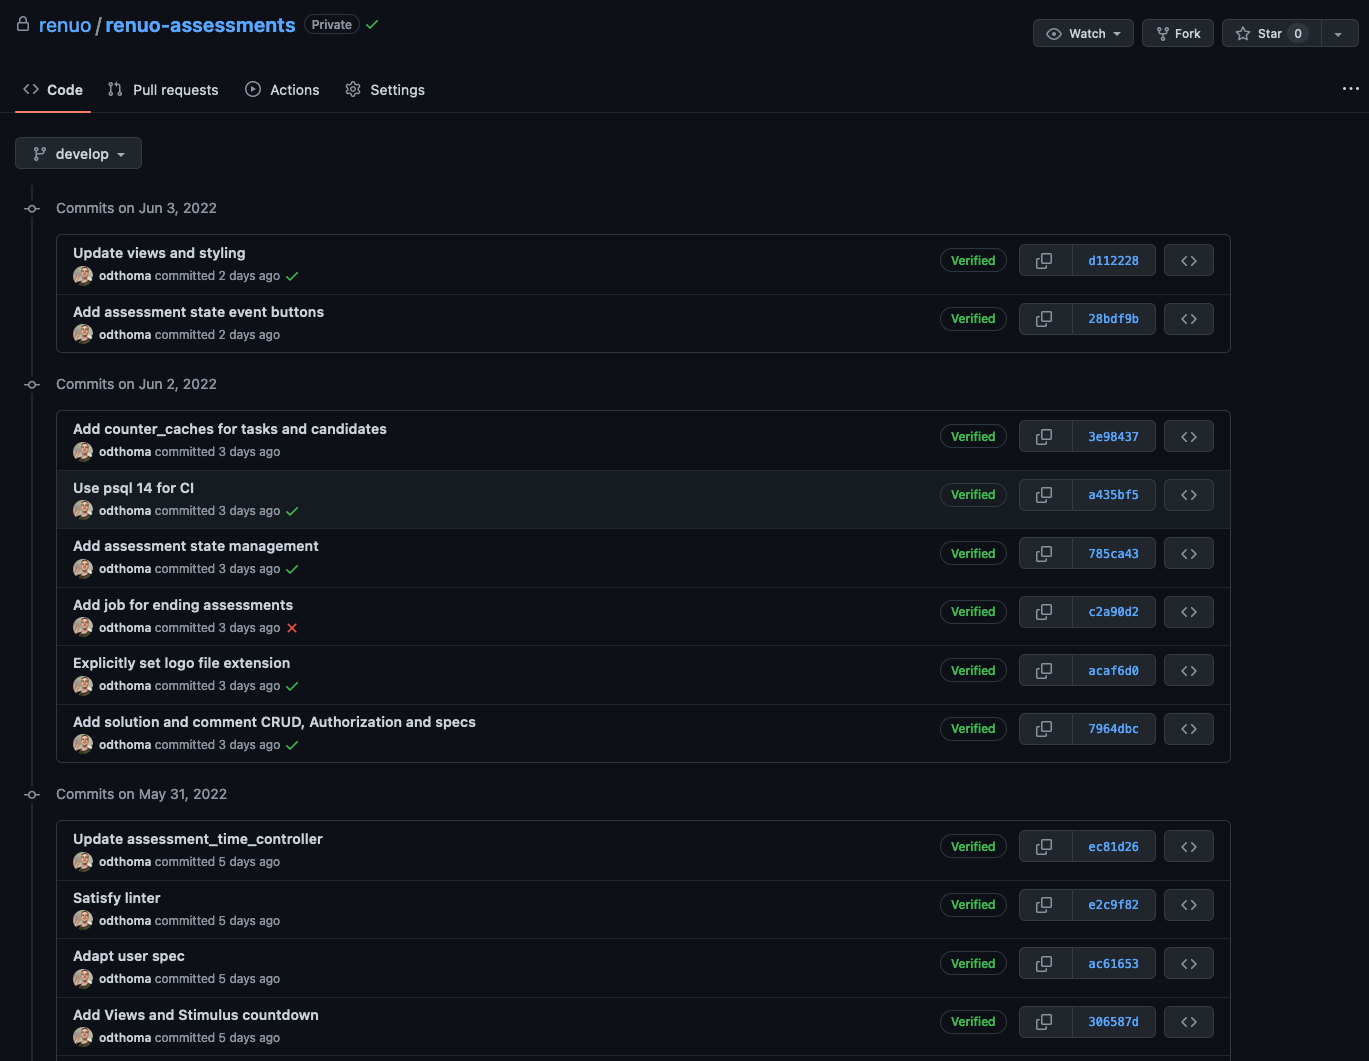
\includegraphics[width=\textwidth]{images/renuo-assessments-github.png}
    \caption{\label{fig:renuo-assessments-github}Ausschnitt der GitHub Commit-History vom Ruby on Rails Projekt}
\end{figure}

\newpage

\subsection{IPA-Bericht}

Das LaTeX Projekt wird ebenfalls in einem Git-Repository versioniert und es werden zu sinnvollen Zeitpunkten Commit gemacht. Diese werden dann regelmässig auf ein Remote (GitHub) gepusht und es wird jeden Abend ein neuer Git-Tag erstellt.
Durch einen \emph{GitHub-Workflow} wird vollautomatisch für jede Version ein PDF generiert.
In dem Repository befinden sich alle Diagramme und sonstigen Dateien, die für die Umsetzung des IPA-Berichtes notwendig sind. 
So ist eine rasche Wiederherstellung der aktuellen Daten im Falle eines Datenverlustes jederzeit und von überall aus möglich.

\begin{figure}[H]
    \centering
    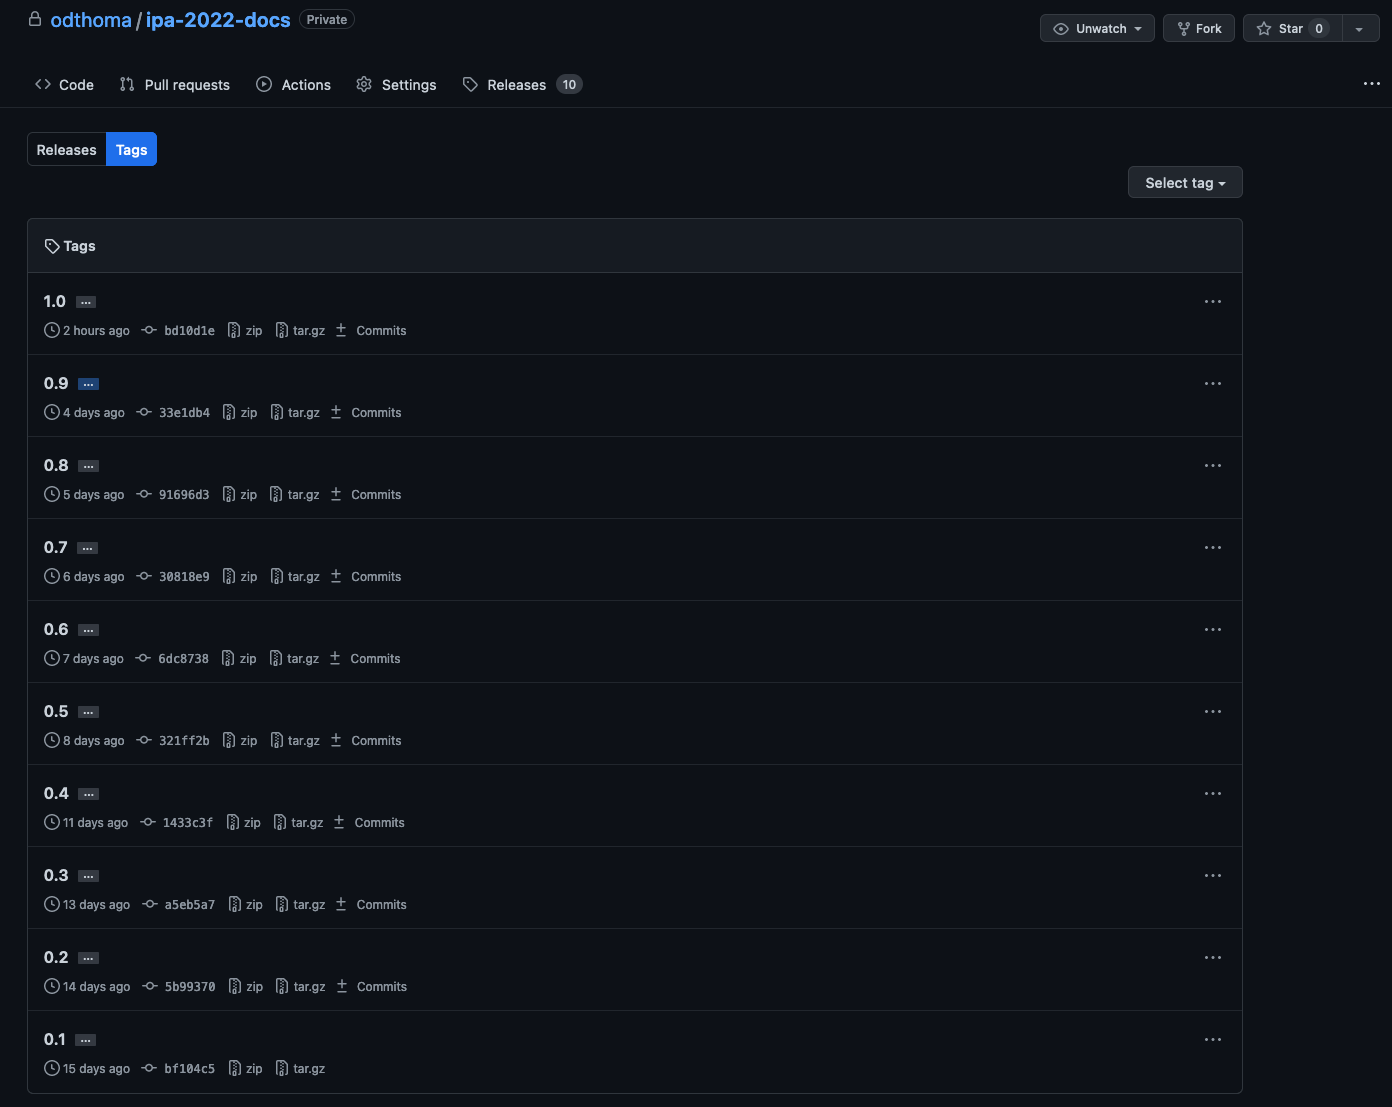
\includegraphics[width=\textwidth]{images/latex-github-tags.png}
    \caption{\label{fig:latex-github-tags}Tägliche Versionierung des IPA-Berichts über Git-Tags}
\end{figure}
